\documentclass{article}
\usepackage[T1]{fontenc} 
\usepackage[utf8]{inputenc}
\usepackage[french]{babel}
\usepackage{listings, xcolor, graphicx}
\usepackage{amsmath}
\usepackage{textgreek}
\usepackage{enumitem}
\graphicspath{ {./} }

\title{Modélisation de la propagation des variants du COVID}
\author{BOUZAKRI Wassim \\COUPET Joss \\MARCHETTI Marie-Eden \\VASSEUR Pierre-Adrien}
\date{Février 2022}

\begin{document}

\maketitle

\section{Résumé}

Dans ce rapport, ...

\section{Introduction}

Dans ce rapport, on va étudier la propagation de la Covid-19 par le biais des variants.
On se demande alors si leur circulation et mutation influencent le comportement de l'épidémie, en plus de considérer leur interaction entre eux.\\

\noindent
Concernant les recherches existantes, on a découvert peu d'articles présentant des simulations de propagation de la Covid-19 par le biais des variants.
Les quelques articles existants se concentraient surtout des propriétés biologiques du virus influencant la simulation de la mutation et la propagation.
Par exemple, la taille du génome du virus parent ou les symptômes. (Marquioni \& de Aguiar, 2021), ce sont des analyses intéressantes mais sans doute trop complexe sans avoir suivi la formation adéquate.\\

\noindent
Une approche différente et plus simple a été choisie afin de permettre la compréhension par un maximum de lecteurs. Elle sere détaillée tout au long de cet article.\\

\noindent
Tout d'abord, on présentera la modélisation de départ de la propagation de la Covid-19 initialisée avec un seul variant. \par
Ensuite, on se penchera sur la modélisation plus complexe initialisée avec deux variants, sur lequel on concentra notre étude.\par
Puis, on réalisera plusieurs simulations différentes dans l'objectif d'interpréter le comportement de ce modèle grâce aux résultats.\par
Enfin, on concluera notre étude.\\

\section{Modélisation de départ}

La modélisation de départ est très basique et représente l'évolution d'un seul variant en prenant en compte sa virulence et sa force de contamination.\\
\noindent
Les variables de base pour seulement 1 virus sont les suivantes : 
\begin{align}
    S(t)= \text{\% de personnes saines dans la population au temps t} \\
    I(t)= \text{\% de personnes contaminées dans la population au temps t} \\
    R(t)= \text{\% de personnes en rémission dans la population au temps t} \\
\end{align}
\noindent
\textalpha \space représente la force de contagion du virus. \\
\textbeta \space représente la virulence du virus. \\
\noindent
La simulation discrétisée par le temps est représentée dans le système d'équation suivante : 
\begin{align}
    \dot{S}(t)= -\alpha S(t)I(t) \\
    \dot{I}(t)= \alpha S(t)I(t)-\beta I(t) \\
    \dot{R}(t)= \beta I(t) + \beta I(t)
\end{align}
\noindent
Cette mise en équation permet de simuler facilement la propagation de la Covid-19 au sein d'une population saine.\\

\section{Modélisation avancée}

Afin de modéliser un modèle à X variants, un nouveau système d'équation est nécessaire.\\ 
Pour débuter, on a définit un nouveau modèle avec 2 variants qui pourra être modifié pour permettre de simuler X variants.\\
\noindent
Les variables de notre nouveau modèle sont les mêmes que précédemment, c'est-à-dire :
\begin{align}
    S_1(t)= \text{\% de non infecté par le variant 1.} \\
    S_2(t)= \text{\% de non infecté par le variant 2.} \\
    I_1(t)= \text{\% d'infecté au variant 1.} \\
    I_2(t)= \text{\% d'infecté au variant 2.} \\
    R_1(t)= \text{\% de remis au variant 1.} \\
    R_2(t)= \text{\% de remis au variant 2.} \\
\end{align}
\noindent
On obtient donc 2 systèmes d'équations différents. \\
\noindent
Le premier système d'équation est celui qui permet de simuler l'évolution du premier variant.\\
\begin{align}
    \dot{S_1}(t)= -\alpha_1 S_1(t)I_1(t) \\
    \dot{I_1}(t)= \alpha_1 S_1(t)I_1(t)-\beta_1 I_1(t) \\
    \dot{R_1}(t)= \beta_1 I_1(t)
\end{align}
On obtient le même pour le second variant. \\
Cependant le système est trop simple, il n'y a pas d'interaction entre les virus. \\
On fait donc un nouveau système qui permet une interaction entre les variants et qui sera adaptable à X variants à l'aide de boucle en programmation :
\begin{align}
    \dot{S}(t)= -\alpha_1 S(t)I_1(t) - \alpha_2 S(t)I_2(t) \\
    \dot{I_1}(t)= \alpha_1 S(t)I_1(t)-\beta_1 I_1(t) \\
    \dot{I_2}(t)= \alpha_2 S(t)I_2(t)-\beta_2 I_2(t) \\
    \dot{R}(t)= \beta_1 I_1(t) + \beta_2 I_2(t)
\end{align}
\noindent
Lors de la création de ce modèle, on a définit les règles suivante : \\
\begin{enumerate}
    \item On ne peut être infecté que par un variant à la fois. \\
    \item Après s'être remis, on ne peut plus être infecté par un variant. \\
\end{enumerate}

\noindent
On veut maintenant modéliser les mutations.\\
Le \% de chance de mutation du variant 1 sur l'intervalle de temps T est défini par :
\begin{align}
    mut = I_1(t)*(1-e^{\gamma T})\text{ avec }\gamma > \text{0}
\end{align}
\noindent
Si une mutation doit être réalisé alors \\
\noindent
T est un nombre aléatoire tel que 0 < T < 100 \\
t est la probabilité que les propriétés d'un variant soient fortement différentes des propriétés du parent.\\
Si T > t \\
Alors F(T) = 
\begin{align}
    new_\alpha = x, \alpha_{variant} \times 1.2 < x < \alpha_{variant} \times 1.4 \\
    new_\beta = x, \beta_{variant} \times 0.9 < x < \beta_{variant} \times 1.1
\end{align}
\noindent
Sinon F(T) = \\
\begin{align}
    new_\alpha= x, \alpha_{variant} \times 0.1 < x < \alpha_{variant} \times 1.9 \\
    new_\beta= x, \beta_{variant} \times 0.1 < x < \beta_{variant} \times 1.9
\end{align}


\section{Simulations numériques}

Dans cette partie, on va réaliser plusieurs simulations avec différents paramètres. Ces simulations sont produites avec un outil que l'on a développé et déployé en ligne, disponible à l'adresse suivante : https://modelisation.vercel.app/ \\
Les paramètres sont les suivants : \\
\begin{enumerate}
    \item Taux de personnes saines -> 0,97
    \item Taux de personnes en rémission -> 0
    \item Gamma pour la probabilité de mutation du virus -> 0,01
    \item Probabilité de créer un nouveau variant avec des paramètres très éloignées de son parent -> 1
    \item Durée de la simulation en jours -> 2000\\
\end{enumerate}
Pour le variant 1 : 
\begin{enumerate}
    \item Taux de personnes infecté -> 0,01
    \item Force de contagation du virus -> 0,01
    \item Virulence du virus -> 0,001\\
\end{enumerate}
Pour le variant 2 : 
\begin{enumerate}
    \item Taux de personnes infecté -> 0,02
    \item Force de contagation du virus -> 0,01
    \item Virulence du virus -> 0,005\\
\end{enumerate}

\subsection{Simulation 1}

\begin{figure}[h]
    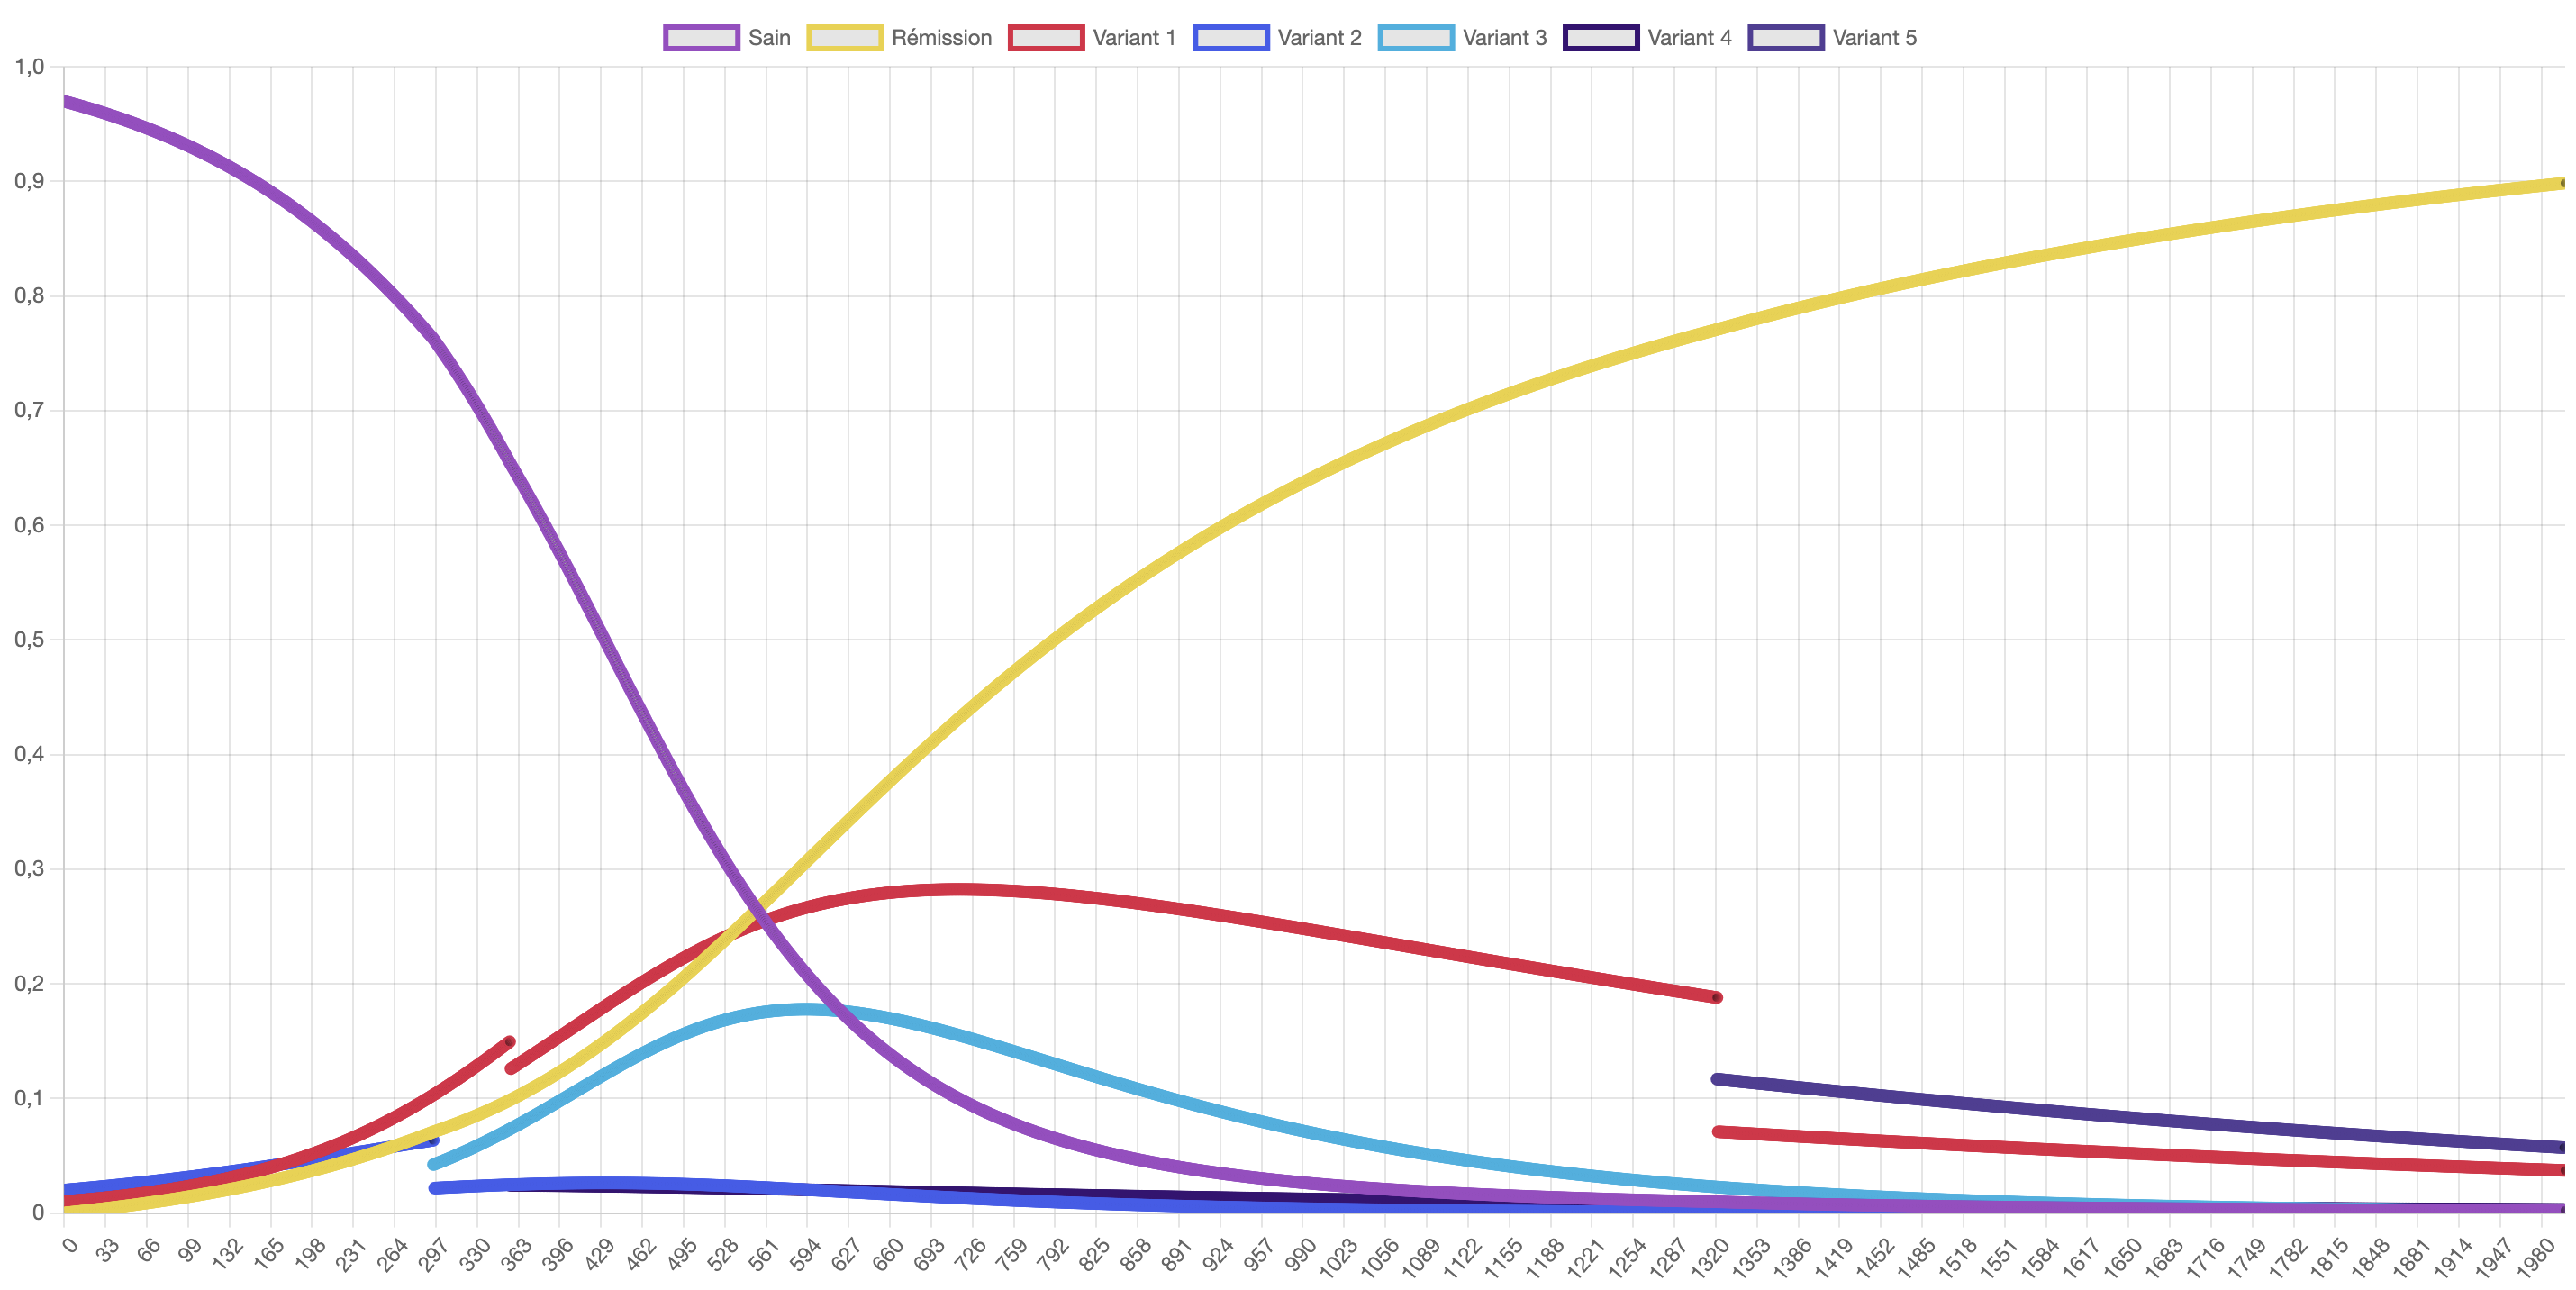
\includegraphics[width=\linewidth]{images/Simulation1.png}
    \caption{Simulation 1}
    \label{fig:simulation1}
\end{figure}

\noindent
La simulation actuelle utilise les paramètres de base énoncé un peu plus haut. \\

\begin{enumerate}
    \item Variant 3 : Apparition au jour 297. Il est issu du variant 2. Il touche un taux plus important de la population comparé à son parent. Il survit plus longtemps et est plus contagieux.
    \item Variant 4 : Apparition au jour 363. Il est issu du variant 1. Il ne survit pas.
    \item Variant 5 : Apparition au jour 1320. Il est issu du variant 1. Il survit jusqu'à la fin de la simulation avec un taux de contagion supérieur aux autres variants. \\
\end{enumerate}


\subsection{Simulation 2}
...
\subsection{Simulation 3}
...
\subsection{Simulation 4}
.......

\section{Interprétation des résultats}

On remarque que les nouveaux variants entrainent une coupure dans les courbes des variants dont ils sont issus. \\ 
En effet, le taux de personnes infecté par un variant est issu du taux de personne infecté par le variant parent. \\

L'effet de la durée de la simulation sur les variants (à la fin, est-ce qu'un variant domine ou alors est-ce que tout le monde est remis ?) \\

Sur un temps T défini, résultats :\\
- apparition de nouveaux variants par mutations, nombre final de variants\\
- impact sur les personnes saines, en rémission\\
- mutation qui prend le dessus sur son variant père (extraire caractéristiques)\\

\section{Conclusion}

reprendre la problématique, réponse\\

Concernant les perspectives d'améliorations, nous pouvons envisager :
\begin{enumerate}
    \item La gestion du nombre de variants de départ. Cela permettrait d'approfondir encore plus les possibilité de simulation. 
    \item L'ajout d'une notion de graine lié au randomisateur. Avec cela, on peut s'assurer que les résultats obtenus sont toujours identiques pour les mêmes paramètres bien que l'on utilise un système se basant sur une forme d'aléatoire. 
    \item La possibilité de se faire infecter par plusieurs variants en même temps. 
    \item La possibilité de se faire infecter une nouvelle fois après guérison d'un autre variant. 
    \item L'ajout d'une notion de vaccination, les personnes saines pourraient être vaccinées ou non ainsi que les personnes remises. 
\end{enumerate}

\section{Référence}

Marquioni, V., & de Aguiar, M. (2021). Modeling neutral viral mutations in the spread of SARS-CoV-2 epidemics. PLOS ONE, 16(7), e0255438. doi: 10.1371/journal.pone.0255438


\end{document}
